\documentclass[conference]{IEEEtran}
\IEEEoverridecommandlockouts

\usepackage{cite}
\usepackage{amsmath,amssymb}
\usepackage{graphicx}
\usepackage{booktabs}
\usepackage{multirow}
\usepackage{xcolor}
\usepackage[hidelinks]{hyperref}

\newcommand{\A}[1]{\textsf{#1}}                         % arm identifiers
\newcommand{\pending}[1]{\textcolor{red}{[PENDING: #1]}} % result not yet run
\newcommand{\pmsd}[1]{{\scriptsize$\pm$#1}}

\begin{document}

\title{Just Keep Pretraining: Unlabeled Headlines Beat GANs, Helper Tasks and LLM Data for Low-Label Sarcasm Detection}

% Double-blind submission: no author names, affiliations or links.
\author{\IEEEauthorblockN{Anonymous Authors}
\IEEEauthorblockA{\textit{Affiliation withheld for review}}}

\maketitle

\begin{abstract}
Semi-supervised sarcasm detectors combine several ways of using unlabeled text, such as GAN-BERT with sentiment and emotion helper tasks, and report their gains as a whole. We compare these routes one at a time in a single controlled testbed on the News Headlines dataset, with the same encoder, step budget and test protocol, label budgets from 1\% to 100\%, five seeds, paired bootstrap tests and predictions fixed before each experiment. The routes are a GAN, a diffusion model used as generator or as a consistency augmenter, LLM-written headline pairs, helper heads, adversarial training (FGM), self-training, and two self-supervised objectives that continue pretraining BERT on the unlabeled training headlines: masked language modeling (MLM) and a JEPA-style latent prediction objective. The simplest route wins clearly. MLM pretraining raises macro-F1 by 7.4 points at 1\% labels and 2.8 points at 10\%, stable across three pretraining runs. With 1\% of the labels, it scores level with plain BERT trained on 10\%. The GAN and diffusion fakes add nothing, diffusion consistency and LLM-written data hurt, and helper heads, FGM and self-training give about 1.6 points each at 1\%. On top of the pretrained encoder, these three add nothing significant alone and 1.0 point together at 1\%. The gain is in label efficiency, not in sarcasm understanding: pretrained models rely on outlet-specific words as much as BERT does, and none transfers to iSarcasmEval.
\end{abstract}

\begin{IEEEkeywords}
sarcasm detection, semi-supervised learning, task-adaptive pretraining, label efficiency, GAN-BERT, controlled comparison
\end{IEEEkeywords}

% ======================================================================
\section{Introduction}

Sarcasm says the opposite of what it means, so systems that read surface sentiment fail on it, and labeled sarcasm data are expensive to collect. Semi-supervised learning promises to make up for few labels with plenty of unlabeled text. A recent model for the News Headlines dataset~\cite{misra2023sarcasm} combines GAN-BERT~\cite{croce2020ganbert}, which learns from unlabeled text through a generator--discriminator game, with sentiment and emotion helper tasks whose labels come from pretrained classifiers, and reports 93.88\% accuracy~\cite{irfan2025seed}.

Such systems use unlabeled text in one particular way and report the result as a whole. Many other ways exist: generating extra data, adding helper targets, perturbing the input, labeling the unlabeled text with the model itself, or simply continuing BERT's own pretraining on it. Task-adaptive pretraining (TAPT)~\cite{gururangan2020dont} is known to help most when labels are few, and a recent comparison on topic and sentiment tasks found it more robust than five self-training methods~\cite{shi2023rethinking}. For sarcasm, and for this dataset, these routes have not been compared under one protocol.

We compare ten routes to the same unlabeled headlines in a single testbed, in which only the route under test changes. We ask three questions: (Q1) which route gives the largest gain when labels are scarce; (Q2) is that gain stable, and how many labels does it save; (Q3) does it reflect better sarcasm detection, or something narrower?

Our contributions are: (i) a controlled comparison of ten routes, including a GAN, a diffusion model, LLM-written pairs, helper tasks, FGM, self-training and two self-supervised pretraining objectives, at budgets from 1\% to 100\% with paired bootstrap tests and predictions fixed in advance; (ii) evidence that plain MLM pretraining on the unlabeled training headlines beats every other route, is stable across pretraining runs, and absorbs the gains of the other routes; (iii) checks that bound the claim: the gain is in label efficiency on this dataset, with no change in reliance on outlet words and no transfer to author-labeled sarcasm.

% ======================================================================
\section{Related Work}

\textbf{Semi-supervised text classification.} GAN-BERT~\cite{croce2020ganbert} adds a generator of fake sentence vectors and a $(k{+}1)$-way discriminator trained with feature matching~\cite{salimans2016improved}. Self-training labels unlabeled data with the model's own confident predictions~\cite{lee2013pseudo}; consistency training asks for the same prediction on perturbed inputs~\cite{xie2020uda}. Semi-supervised methods can look better than they are when baselines are weak~\cite{oliver2018realistic}. Continued pretraining on the task's own unlabeled text~\cite{gururangan2020dont} was found to be a stronger and more robust semi-supervised learner than self-training on general classification tasks~\cite{shi2023rethinking}. We test whether this holds for sarcasm, against a wider set of routes, including the ones used by recent sarcasm systems.

\textbf{Affect and sarcasm.} Sentiment and emotion have been used as auxiliary tasks for sarcasm~\cite{chauhan2020sentiment}, as intermediate tasks for BERT~\cite{savini2022intermediate} and as lexicon-based soft targets~\cite{chen2022jointly}; the combined GAN and multi-task model~\cite{irfan2025seed} uses them with labels from pretrained classifiers~\cite{barbieri2020tweeteval,demszky2020goemotions}. FGM~\cite{miyato2017adversarial} was reported to match GAN-BERT for Bengali sarcasm~\cite{zihan2026fgm}.

\textbf{Shortcuts and transfer.} In News Headlines the label equals the outlet (\textit{The Onion} vs.\ \textit{HuffPost}), a known source of shortcut learning~\cite{gururangan2018annotation,geirhos2020shortcut}, and sarcasm detectors transfer poorly across datasets~\cite{jang2024generalizable}.

% ======================================================================
\section{Experimental Design}

\subsection{Data and label budgets}
\textbf{News Headlines}~\cite{misra2023sarcasm}: after removing punctuation~\cite{irfan2025seed} and 118 duplicates, 28,501 headlines remain (47.5\% sarcastic), split into 22,800 training, 2,850 development and 2,851 test headlines. For each seed we draw nested labeled subsets $L$ of 1, 5, 10, 30 and 100\% of the training set (228 to 22,800 headlines); the rest is the unlabeled pool $U$, whose labels are hidden. \textbf{iSarcasmEval}~\cite{abufarha2022semeval} (English Task~A, 1,400 test tweets labeled by their authors) is used only for transfer.

\subsection{Routes to the unlabeled text}
Every run fine-tunes bert-base-uncased~\cite{devlin2019bert} with a linear sarcasm head on the [CLS] vector. Routes differ only in the switch under test (arm codes in parentheses):
\begin{itemize}
\item \textbf{Baselines}: TF-IDF with logistic regression (\A{A0}); BERT on $L$ only (\A{A1}).
\item \textbf{GAN} (\A{A4}): GAN-BERT~\cite{croce2020ganbert} reading $U$; \A{A5} adds the helper heads below (our re-implementation of the combined model~\cite{irfan2025seed}).
\item \textbf{Diffusion}~\cite{ho2020ddpm}: a denoising model over [CLS] vectors (100 noise levels) whose samples replace the GAN's fakes (\A{A24}), or which perturbs $U$ vectors for a consistency loss (\A{A25}).
\item \textbf{LLM-written pairs} (\A{A10}): 22,417 sarcastic/serious headline pairs written by three open LLMs, added as a second labeled batch.
\item \textbf{Helper heads} (\A{A2}): sentiment and emotion heads trained on $L$ with teacher labels, loss weight 0.3.
\item \textbf{FGM} (\A{A7}): an adversarial perturbation of size $\epsilon{=}0.5$ on the word embeddings~\cite{miyato2017adversarial}; uses $L$ only.
\item \textbf{Self-training} (\A{A6}): the \A{A1} model labels $U$; headlines with confidence $\geq 0.9$ are kept, class-balanced, and a fresh model trains on $L$ plus these.
\item \textbf{Self-supervised pretraining} on the 22,800 training headlines as text, with no labels, before the \A{A1} fine-tuning: \textbf{MLM} (\A{A20}), BERT's masked-word objective (15\% of tokens), and \textbf{JEPA} (\A{A22}), a text adaptation of joint-embedding predictive pretraining~\cite{assran2023ijepa}: two spans covering 25\% of the words are hidden from the encoder, and a small predictor must output the representation that a slowly updated copy of the encoder computes for the full headline. Both run 10,000 steps (batch 64, learning rate $10^{-4}$, 35--44 minutes on one T4 GPU); development and test headlines are never used.
\end{itemize}
Combinations are named in the text. Settings tuned on development data at 10\% labels (learning rate $5{\times}10^{-5}$, helper weight, $\epsilon$) were frozen before any test score was computed; nothing else was tuned.

\subsection{Training and statistics}
All runs use AdamW, 10\% warm-up then linear decay, batch size 32, maximum length 48 and the same step budget, $\max(200, 10 \text{ passes over } L)$, with no early stopping. Seeds 0--4 change the labeled subset, initialization and batch order; training is deterministic, and repeated runs reproduced earlier predictions exactly. We report test macro-F1 (mean $\pm$ s.d.\ over seeds). Two routes are compared with a paired bootstrap over test headlines~\cite{berg2012empirical} (10,000 resamples, the same resample for all seeds, difference of seed-averaged scores, 95\% interval), with Holm's correction~\cite{holm1979simple} inside each pre-planned family of contrasts. The predictions for every experiment were written down before it was run.

% ======================================================================
\section{Results}

\begin{table}[t]
\centering
\caption{Test macro-F1 (\%, mean $\pm$ s.d.\ over 5 seeds). $U$: reads the unlabeled pool. Bold: best per budget.}
\label{tab:main}
\footnotesize
\setlength{\tabcolsep}{4pt}
\begin{tabular}{llcc}
\toprule
Arm & Route & 1\% (228) & 10\% (2,280) \\
\midrule
\A{A0} & TF-IDF + logistic regression & 69.7\pmsd{0.7} & 78.1\pmsd{0.6} \\
\A{A1} & BERT & 80.4\pmsd{1.2} & 88.2\pmsd{0.3} \\
\midrule
\A{A4} & GAN-BERT ($U$) & 80.5\pmsd{1.6} & 88.1\pmsd{0.4} \\
\A{A5} & GAN-BERT + helper heads ($U$) & 78.1\pmsd{2.7} & 88.4\pmsd{0.3} \\
\A{A24} & Diffusion fakes ($U$) & 80.3\pmsd{2.8} & 88.0\pmsd{0.6} \\
\A{A25} & Diffusion consistency ($U$) & 75.6\pmsd{4.8} & 87.4\pmsd{0.5} \\
\A{A10} & LLM-written pairs & 64.0\pmsd{0.9} & 73.4\pmsd{0.7} \\
\A{A2} & Helper heads on $L$ (H) & 82.1\pmsd{0.6} & 88.4\pmsd{0.4} \\
\A{A7} & FGM (F) & 82.0\pmsd{0.6} & 89.8\pmsd{0.2} \\
\A{A6} & Self-training, S ($U$) & 82.0\pmsd{0.8} & 88.8\pmsd{0.3} \\
\A{A30} & H + F + S ($U$) & 84.6\pmsd{0.9} & 89.9\pmsd{0.4} \\
\midrule
\A{A22} & JEPA pretraining ($U$) & 86.1\pmsd{0.3} & 89.9\pmsd{0.2} \\
\A{A20} & MLM pretraining ($U$) & 87.8\pmsd{0.6} & 91.0\pmsd{0.3} \\
\A{A36} & MLM + H + F + S ($U$) & \textbf{88.8}\pmsd{0.3} & \textbf{91.6}\pmsd{0.3} \\
\bottomrule
\end{tabular}
\end{table}

\begin{figure*}[t]
\centering
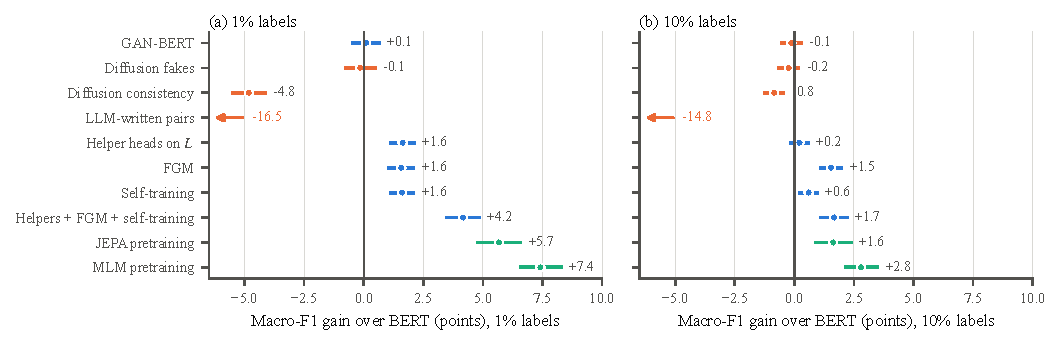
\includegraphics[width=\textwidth]{figures/fig_methods.pdf}
\caption{Q1: gain in test macro-F1 over BERT (\A{A1}) for each route, paired bootstrap over test headlines, 95\% intervals, 5 seeds. Green: self-supervised pretraining on the unlabeled training headlines. The LLM-written pairs fall off the scale.}
\label{fig:methods}
\end{figure*}

\subsection{Q1: Which route gives the gain?}
Table~\ref{tab:main} and Fig.~\ref{fig:methods} give the answer.

\textbf{Generating data does not help.} GAN-BERT is level with BERT at every budget ($+0.10$ points at 1\%, $-0.13$ at 10\%, both $p > 0.5$), and a development-only check of its generator learning rate and of three times more training steps did not change this. Replacing the GAN's fakes with samples from a diffusion model changes nothing ($-0.15$ and $-0.24$), and using the diffusion model to perturb $U$ for a consistency loss costs 4.8 points at 1\% and 0.8 at 10\% (both robust). LLM-written headline pairs cost 16.5 and 14.8 points; a likely reason is that the generated sarcastic headlines differ from real ones in length and stock phrasing, which the model can learn instead of sarcasm. Combining the GAN with helper heads costs 2.3 points at 1\% ($p < 10^{-4}$), with a large seed spread.

\textbf{Three simple routes give about 1.6 points each at 1\%.} Helper heads on $L$ ($+1.63$), FGM ($+1.58$) and self-training ($+1.62$) all help when labels are scarce (all $p < 10^{-4}$). At 10\% only FGM keeps its gain ($+1.55$). Stacking all three gives $+4.17$ at 1\% and $+1.67$ at 10\%, about 86\% of the summed single gains at 1\%.

\textbf{Continued pretraining on the unlabeled headlines is far stronger.} MLM pretraining adds $+7.42$ points at 1\% [6.55, 8.32] and $+2.80$ at 10\% [2.09, 3.53], every seed ahead. The JEPA objective also helps ($+5.67$ and $+1.63$) but trails MLM by 1.75 and 1.17 points (both robust, every seed behind), although it ran for the same number of steps. Predicting masked words beats predicting hidden representations here. MLM alone also beats the stack of the three simple routes, by 3.2 points at 1\% (difference of means).

\subsection{Q2: Is the gain stable, and how many labels does it save?}

\begin{figure}[t]
\centering
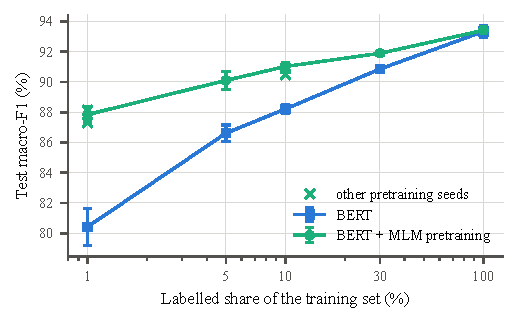
\includegraphics[width=\columnwidth]{figures/fig_curve.pdf}
\caption{Q2: test macro-F1 against the label budget (log scale), mean $\pm$ s.d.\ over 5 seeds. Crosses: MLM pretraining repeated with two other pretraining seeds.}
\label{fig:curve}
\end{figure}

\textbf{Stability.} One pretraining run could be lucky, so we pretrained twice more with different seeds. The three encoders give $+7.42$, $+7.72$ and $+6.89$ points over BERT at 1\% and $+2.80$, $+2.68$ and $+2.26$ at 10\% (all robust, every fine-tuning seed ahead); their mean F1 at 1\% spans only 0.83 points (Fig.~\ref{fig:curve}).

\textbf{Label efficiency.} The gain shrinks as labels grow: $+3.49$ at 5\%, $+1.04$ at 30\% (both robust) and $+0.09$ with every label (not significant). With 1\% of the labels, the pretrained model is level with BERT trained on 10\% ($-0.38$ [$-1.15$, 0.41]); with 10\%, it is level with BERT on 30\% ($+0.17$). Reading BERT's curve at the pretrained model's scores, the same F1 would need 8.5, 4.4, 3.3 and 1.7 times more labels at 1, 5, 10 and 30\%. These are ``no significant difference'' results, not proofs of equality; the intervals are about $\pm 0.8$ points.

\subsection{Does anything add on top of pretraining?}
We repeated the full $2{\times}2{\times}2$ combination of helper heads, FGM and self-training on the MLM-pretrained encoder (Table~\ref{tab:stack}).

\begin{table}[t]
\centering
\caption{Each combination of helper heads (H), FGM (F) and self-training (S), on BERT and on the MLM-pretrained encoder. Test macro-F1 (\%), mean over 5 seeds.}
\label{tab:stack}
\footnotesize
\setlength{\tabcolsep}{5pt}
\begin{tabular}{lcccc}
\toprule
 & \multicolumn{2}{c}{1\% labels} & \multicolumn{2}{c}{10\% labels} \\
\cmidrule(lr){2-3}\cmidrule(lr){4-5}
Added routes & BERT & MLM & BERT & MLM \\
\midrule
none & 80.4 & 87.8 & 88.2 & 91.0 \\
H & 82.1 & 88.3 & 88.4 & 91.1 \\
F & 82.0 & 87.8 & 89.8 & 91.2 \\
S & 82.0 & 88.2 & 88.8 & 91.1 \\
H + F & 83.0 & 88.3 & 89.5 & 91.3 \\
H + S & 83.1 & \textbf{88.9} & 89.2 & 91.1 \\
F + S & 83.9 & 88.5 & 90.3 & 91.5 \\
H + F + S & 84.6 & 88.8 & 89.9 & \textbf{91.6} \\
\bottomrule
\end{tabular}
\end{table}

On the pretrained encoder, no route adds a significant gain on its own (helper heads $+0.48$, $p_{\mathrm{Holm}} = 0.09$; FGM $-0.09$; self-training $+0.35$). Pretraining shrinks each route's gain by 1.1 to 1.7 points at 1\% (all robust interactions). Self-training is not broken: the pretrained teacher's pseudo-labels are 92--96\% correct when checked against the hidden training labels. It simply has little left to teach, because the pretrained model already classifies those headlines. Combined, the routes still add a small, robust amount at 1\%: helper heads with self-training $+1.05$ [0.55, 1.56], all three $+0.97$ [0.39, 1.54]. At 10\% no combination survives correction (all three $+0.58$, $p_{\mathrm{Holm}} = 0.20$). The best recipe at 1\% thus reaches 88.8--88.9 against BERT's 80.4, and about 7.4 of those 8.4 points come from pretraining.

\subsection{Why do helper tasks barely help?}
The helper heads are the core of the multi-task design~\cite{irfan2025seed}, so their weak effect deserves a closer look. Three findings point the same way. First, when the helper labels are shuffled across headlines, the helper heads still add $+1.17$ points at 1\% (robust), 72\% of their gain with real labels; real labels add only 0.46 points over shuffled ones ($p = 0.034$, not robust to correction). Second, the helper labels carry almost no sarcasm signal: a logistic probe on the teacher's eight sentiment and emotion probabilities predicts sarcasm with an AUC of 0.546, and the sentiment teacher agrees only weakly with a 200-headline human audit ($\kappa = 0.24$). Third, on the pretrained encoder their effect is no longer significant. The helper heads act mainly as a regularizer of the shared encoder when labels are very scarce, not as a source of affective knowledge.

\textbf{Polarity flips.} Sarcasm often pairs positive surface sentiment with a negative intent, which could make a sentiment helper pull the encoder the wrong way on exactly those headlines. The test set has 107 sarcastic headlines whose teacher sentiment is positive (474 negative, 774 neutral). \pending{compare the error rate of the helper-head arms (A2, A31) with A1/A20 on these 107 headlines against the other sarcastic headlines, paired bootstrap; CPU analysis on existing predictions. The group is small, so the result is exploratory.}

\subsection{Q3: Better sarcasm detection, or better use of this dataset?}
\textbf{Outlet words.} In News Headlines the label is the outlet. We masked the 200 words most indicative of each outlet (chosen on the training set before any masked score was seen) and, as a control, the same number of random words. Every BERT model loses about 3 points more under cue masking than under random masking. The pretrained models show the same gap: the difference from BERT is $-0.07$ at 1\% and $-0.17$ at 10\%, and no pretrained or stacked arm differs significantly. Pretraining makes the model better at this dataset; it does not make it rely less on outlet vocabulary.

\textbf{Transfer.} On iSarcasmEval, all pretrained arms stay near chance (ROC-AUC 47.8 to 57.3), 11 to 21 points below a baseline that scores each tweet by its word count alone (68.7), and below a BERT model trained on iSarcasmEval itself (65.8). Pretraining on headlines does not carry over to author-labeled sarcasm on Twitter.

% ======================================================================
\section{Discussion}

\textbf{What to use when labels are scarce.} Before building generators, helper tasks or synthetic data, continue pretraining the encoder on the unlabeled text that is already there. In our testbed this costs about 35 minutes of one GPU, needs no extra model or data, and beats every other route by a wide margin. The other routes either add nothing (GAN, diffusion fakes), hurt (diffusion consistency, LLM-written pairs, GAN with helper heads at 1\%), or give gains that pretraining absorbs (helper heads, FGM, self-training). This agrees with what was reported for topic and sentiment tasks~\cite{gururangan2020dont,shi2023rethinking}; the new evidence is that it holds for sarcasm, against the routes used by recent sarcasm systems.

\textbf{What the gain means.} The gain is label efficiency on News Headlines. The pretrained model learns the dataset faster, including its outlet vocabulary, and it does not transfer. High scores on this dataset should not be read as sarcasm understanding.

\textbf{Limitations.} (i) One encoder size, one main dataset and one transfer set; MLM and JEPA used fixed settings, and three pretraining seeds were run for MLM but one for JEPA. (ii) Our GAN and multi-task model is a re-implementation with shared helper heads; the original code was unavailable, so our absolute numbers are not comparable with the reported 93.88\%, which also used 70\% of the labels~\cite{irfan2025seed}. % CHECK 70%: from the seed paper's abstract via a search index, not the full text (iii) Cross-budget comparisons pair different labeled subsets; the bootstrap resamples test headlines only. (iv) The human audit has a single annotator.

% ======================================================================
\section{Conclusion}

Among ten ways to use unlabeled headlines for low-label sarcasm detection, tested under one protocol, the simplest is the best: continue BERT's masked-word pretraining on the unlabeled training text, then fine-tune. It adds 7.4 macro-F1 points with 1\% of the labels, matches plain BERT trained on ten times more labels, is stable across pretraining runs, and leaves little for GANs, helper tasks, FGM or self-training to add. Its gain is in label efficiency on the dataset, not in sarcasm understanding that transfers. Future sarcasm systems should report this baseline before claiming gains from more complex semi-supervised designs, and should evaluate on data whose labels are not tied to the source.

\bibliographystyle{IEEEtran}
\bibliography{refs}

\end{document}
